\documentclass[11pt]{article}
\bibliographystyle{ieeetr}

\usepackage[a4paper, margin=2.0cm]{geometry}
\usepackage{amsmath}
\usepackage{enumitem}
\usepackage{comment}
\usepackage{graphicx}
\usepackage{booktabs}
\usepackage{float}
\usepackage{array}
\usepackage{diagbox}
\usepackage[table]{xcolor}
\usepackage{hyperref}
\usepackage{titlesec}
\usepackage{enumitem}
\usepackage{amsfonts}
\usepackage[skip=4pt]{caption}
\usepackage{hyperref}

\titlespacing*{\section}{0pt}{8pt}{4pt}
\titlespacing*{\subsection}{0pt}{8pt}{4pt}
\setlist[itemize]{itemsep=0pt}
\setlength{\floatsep}{2pt}
\setlength{\textfloatsep}{2pt}
\setlength{\intextsep}{2pt}

\title{\vspace{-1.0cm}Reinforcement Learning Homework 3}
\author{Santoso Alvin Christopher 20265011 \\
\href{https://github.com/alvinsnt/reinforcement-learning-experiments}{GitHub}
}


\date{}

\begin{document}

\maketitle

\section*{Introduction}

This report investigates reinforcement learning through two contrasting environments: Taxi and Breakout. Taxi is addressed using tabular Q-learning due to its small, discrete, and fully observable state space, allowing efficient and stable learning of optimal policies. Breakout, in contrast, requires Deep Q-Networks (DQN) because it operates on high-dimensional image-based observations that necessitate representation learning through neural networks. The report compares these environments in terms of state representation, action complexity, reward structure, sample efficiency, computational cost, learning stability, and interpretability. It further examines key reinforcement learning methods including Q-learning, SARSA, and DQN, alongside techniques such as $\epsilon$-greedy exploration, experience replay, and target networks. Overall, the study highlights how problem structure fundamentally determines the appropriate learning approach and the associated challenges in training reinforcement learning agents.

\section*{Taxi Environment and Tabular Q-Learning}

\subsection*{Describe the Taxi environment in terms of the following MDP components:}

\begin{itemize}
    \item State space $\mathcal{S}$
    
    The state consists of the taxi’s position (row and column), passenger location (red, green, yellow, blue, in taxi), destination (red, green, yellow, blue). Since there are 25 possible locations in a 5x5 gridworld, 5 possible passenger location, and 4 destination location, there are 500 possible states. However, in an episode there are only 400 states that are visited as states where the passenger's location and destination is the same means episode termination. Moreover, there are four additional states which can be observed after a successful episode where the passenger and taxi are at the destination. This gives a total of 404 reachable discrete states~\cite{towers2024gymnasium}.

    \item Action space $\mathcal{A}$
    
    The action space consists of 6 actions which is represented by an integer in the range {0, 5} indicating which direction to move the taxi or to pickup/drop off passengers. The actions are: move south (0), north (1), east (2), west (3), pickup passenger (4), and drop off passenger (5).~\cite{towers2024gymnasium}

    \item Reward function $R(s, a, s^\prime)$
    \[
    R(s,a,s') =
    \begin{cases}
    +20 & \text{if the passenger is successfully dropped off at the destination} \\
    -10 & \text{if an illegal pickup or dropoff is attempted} \\
    -1  & \text{otherwise (each time step penalty)}
    \end{cases}
    \]

    \item Transition dynamics
    
    Taxi has deterministic transition dynamics where movement actions deterministically change position unless blocked by walls, pickup works only if taxi is at passenger location, and dropoff only works if taxi is at destination with passenger \cite{towers2024gymnasium}.

    \item Terminal condition
    
    The episode ends if the taxi successfully drops off the passenger or when the episode length is 200 \cite{towers2024gymnasium}.

\end{itemize}

\subsection*{Explain why Taxi is suitable for tabular reinforcement learning}

Taxi has a small enough state space to feasibly store Q table, has discrete states and actions which don't require function approximations, is fully observable, and has deterministic transitions

\subsection*{Answer the following questions}

\begin{itemize}
    \item How many states does the Taxi environment have?
    
    400 states

    \item How many actions are available?
    
    6 actions, which are: move south (0), north (1), east (2), west (3), pickup passenger (4), and drop off passenger (5).

    \item Why is this environment considered a discrete MDP?
    
    State space $\mathcal{S}$ is finite, action space $\mathcal{A}$ is finite and discrete, and transitions occur between discrete states, not continuous values

    \item What role do negative rewards play in this environment?
    
    In Taxi, there are two cases where the reward is negative. One is the -1 reward for each time step elapsed, which plays the role of pushing the agent to find the shortest path. The other case where the reward is negative is when the agent takes illegal actions. The reward value for this case is -10 in order to more strongly discourage illegal actions by the agent.
\end{itemize}

\subsection*{Tabular Q-Learning for Taxi}

Here are the results of implementing a Q-Learning algorithm with an $\epsilon$-greedy action selection strategy with $\alpha = 0.9$, $\gamma = 0.9$, and $\epsilon = 0.3$.

\begin{itemize}
    \item Final average reward over the last 100 episodes: -12.26
    \item Average number of steps over the last 100 episodes: 19.22
    \item Training time: 2.81 seconds
    \item Plot: Figure \ref{e0.3}
\end{itemize}

\subsection*{Questions}

\begin{itemize}
    \item Why is Q-learning considered an off-policy method?
    
    Q-learning is considered an off-policy method because it uses a separate behaviour policy which is used to generate data to help optimize the target policy.

    \item What happens if $\epsilon$ is too high?
    
    The agent will take seemingly random actions and might not learn the opimal policy effectively.

    \item What happens if $\epsilon$ is too low?
    
    There is a risk of the agent getting stuck in a local maxima and never learns the truly optimal policy.

    \item How do $\alpha$ and $\gamma$ affect learning?
        
    if the $\alpha$ is too low then the agent will be slower to converge because the update is carried out in smaller values. However, if the $\alpha$ is too high then the agent might not converge.
    
    If the $\gamma$ is too low then the agent will be "myopic" and will more prioritize immediate gains rather than long term cumulative reward. Meanwhile, a $\gamma$ closer too 1, will have the agent put more emphasis or care more about long term cumulative reward.
\end{itemize}

\section*{Improvement of Taxi Agent}

\subsection*{Epsilon Decay}

For the Taxi environment, a decaying $\epsilon$ performs better than a fixed $\epsilon$ because exploration is mainly needed during the early stages of learning. This can be observed by comparing figure \ref{e0.9_nodecay} and figure \ref{e0.9_decay0.0005}. With a fixed high $\epsilon$, the agent continues taking random exploratory actions, reducing the frequency of optimal actions and leading to sub-optimal rewards. In contrast, $\epsilon$-decay allows the agent to explore initially and gradually shift toward exploitation as $\epsilon$ decreases.

The experiments also show that lower $\epsilon$ values achieve higher rewards in the Taxi environment, as seen in figure \ref{e0.9_decay0.0005} and figure \ref{e0.2_decay0.0005}. Since Taxi has a small state and action space, extensive exploration is unnecessary, allowing the agent to converge faster with lower exploration rates. The results further show that $\epsilon = 0$, shown in figure \ref{e0.0}, performs better than higher $\epsilon$ values with/without decay. This is likely because the environment is deterministic, the state space is limited, and negative rewards quickly guide updates in the Q-table, enabling the agent to learn effective policies even without explicit exploration.

\subsection*{SARSA}

Q-Learning updates using the maximum Q-value of the next state, while SARSA updates using the Q-value of the next action actually taken. As a result, SARSA learns more conservatively because it incorporates exploratory actions into its updates, whereas Q-Learning learns faster toward the optimal greedy policy but is more prone to overestimation bias from the max operator.

Using the same learning rate ($\alpha$) and discount factor $\gamma$ of 0.9, SARSA showed greater reward fluctuations and lower performance than Q-Learning over 5000 episodes. Since Taxi is deterministic, small, and low-risk, Q-Learning's optimistic greedy updates perform well. In contrast, SARSA is generally more effective in stochastic or risky environments such as cliff-walking.

When $\epsilon$ is a small value (i.e. 0.1), it is observed that the reward per episode fluctuates less when compared to SARSA with higher $\epsilon$ values. However, when $\epsilon = 0$, SARSA gave comparable performance to Q-Learning. This is because, under $\epsilon = 0$, the selected next action satisfies $a' = arg \max_{a'}Q(s',a')$. Causing the SARSA update target $r + \gamma Q(s',a')$ to become equivalent to the Q-Learning target $r + \gamma \max_{a'} Q(s', a')$ making both update rules effectively identical.

%\[
%Q(s,a)\leftarrow Q(s,a) + \alpha [r + \gamma \max_{a'} Q(s',a')-Q(s,a)]
%.\]

\subsection*{Hyperparameter Study}

In order to compare the effects of interactions between hyperparameters, three experiments are carried out where one of the hyperparameters is fixed while others are varied. For the first, second, and third experiment respectively: $\gamma$ is fixed to 0.9 (figure \ref{alphavsepsilon}); $\epsilon$ is fixed to 0.2 (figure \ref{alphavsgamma}); and $\alpha$ is fixed to 0.3 (figure \ref{epsilonvsgamma}).

From figure \ref{alphavsepsilon} and \ref{alphavsgamma}, it can be seen that even though $\epsilon$ and $\gamma$ are varied, most experiments with $\alpha = 0.0$ is always the lowest with several exceptions such as when $\epsilon = 1.0$ in figure \ref{alphavsepsilon} and when $\gamma = 0.0$ in \ref{alphavsgamma}. From this observation, it can be concluded that for all hyperparameter combinations $\alpha = 0.0$ affects reward adversely.

From figure \ref{alphavsepsilon} and especially in figure \ref{epsilonvsgamma}, it can be seen that for Taxi, an increasing $\epsilon$ value gives worse reward values for all hyperparameter combinations. This fact is also supported by figure \ref{e0.0} where a zero $\epsilon$ value gives best performance in Taxi. Another thing worth noting in figure \ref{epsilonvsgamma} is the fact that $\gamma$ interacts in a similiar way as $\alpha$ in figures \ref{alphavsepsilon} and \ref{alphavsgamma} where they give a positive effect to rewards received as long as they are not equal to zero.

\section*{Breakout Environment and DQN}

\subsection*{Breakout Environment}

\begin{itemize}
    \item Observation Space
    
    According to the official documentation for Arcade Learning Environment \cite{bellemare13arcade}, three observation spaces are available: RGB, RAM, and grayscale. RGB observations provide 210×260 RGB game frames, RAM observations provide 128 bytes of Atari console memory, and grayscale observations provide 210×260 grayscale game frames.

    \item Action Space
    
    The action space of Breakout consists of 4 actions. NOOP (0), FIRE (1), RIGHT (2), LEFT (3) \cite{bellemare13arcade}.

    \item Reward Structure

    The official documentation for Arcade Learning Environment referred the atariage website for the values of points of each brick color \cite{AtariAgeAtari2600}: red and orange 7 points, yellow and green 4 points, aqua and blue 1 point.

    \item Episode Termination Condition
    
    Episode is terminated when all 5 lives in Breakout are lost

\end{itemize}

\subsection*{Taxi and Breakout Comparison}

\begin{itemize}
    \item State Representations
    
    In Taxi, the state space $\mathcal{S}$ is represented by the taxi position, passenger location, and destination, resulting in only 500 states. This relatively small state space makes tabular methods feasible without requiring function approximation.
    
    In contrast, Breakout has a much larger state space, consisting of combinations of image pixels (RGB or grayscale observations) or memory values (RAM observations). Storing all possible states in a Q-table would be impractical due to the enormous number of possible combinations. Therefore, function approximation methods are required for effective learning.

    \item Action Space
    
    Taxi has 6 actions which are: move south, north, east, west, pickup passenger, and drop off passenger. Meanwhile, Breakout has 4 actions which are: NOOP, FIRE, RIGHT, and LEFT.

    It is worth noting that even though the number of actions available in Breakout is smaller than Taxi, choosing the correct actions is significantly more difficult due the more complex state representations and reward sparsity in Breakout.

    \item Reward Sparsity
    
    A major difference between Taxi and Breakout is reward frequency. In Taxi, rewards are dense, with negative rewards given at each timestep and for illegal actions, and positive rewards for successfully delivering the passenger. In contrast, Breakout has sparse rewards, where rewards are only received when blocks are broken, causing many observation frames to produce zero reward.

    \item Difficulty of Exploration
    
    Exploration in Taxi is relatively easy because the reward structure naturally guides the agent toward the optimal policy. Negative rewards for elapsed timesteps and illegal actions encourage the agent to learn the shortest valid path, while positive rewards reinforce correct passenger pickup and drop-off behavior. This is supported by figure \ref{e0.0}, where the agent converges similarly to figure \ref{e0.9_decay0.0005} but faster, suggesting that explicit exploration contributes little in Taxi. In contrast, Breakout has sparse rewards and a very large state space. Random actions rarely produce meaningful rewards, requiring the agent to learn precise action sequences based on the observed state to achieve good performance.

    \item Size of the Learning Problem
    
    Taxi has 500 available states and 6 available actions. In total, a number of 3000 combinations which is still managable to store in memory for tabular solutions. Meanwhile, Breakout consists of a huge number of possible image observations which is not managable to store in memory.

\end{itemize}

\subsection*{Why Q-table is not Practical for Breakout?}

A Q-table stores $Q(s,a)$ for every state-action pair. In breakout, the states are the image frames of Breakout, which are numerous due to every pixel contributing to the amount of states. For tabular solutions like the Q-Table, The sheer amount of image frame combinations would require a very big amount of memory, learning would not be as fast as function approximation methods, and generalization would not be as good as function approximation methods.

\subsection*{Why Function Approximation is Necessary?}

Breakout uses image-based observation where the amount of states is very large due to the number of different pixel combinations contributing to the amount of states. If tabular solutions, where each exact state is memorized, is used, then the memory requirements would be massive and not generalize well.

\subsection*{Why is Image-based Observation more Difficult than Dicrete State Observation?}

In Taxi, the environment directly provides structured information such as the taxi position, passenger location, and destination. In contrast, Breakout only provides raw pixel observations, requiring the agent to infer meaningful features from the images. As a result, Breakout becomes both a perception and control problem, making it significantly more difficult than Taxi, which is primarily a control problem. Additionally, image-based observations in Breakout contain large amounts of irrelevant information, unlike Taxi where only essential state information is provided. This further increases the complexity and size of the effective state representation compared to the compact Q-table used in Taxi.

\subsection*{What Information must the Agent Extract from the Screen?}

In order to effectively learn, the agent must extract information regarding ball position, velocity, and direction, paddle position, brick position, as well as collision dynamics (how the ball bounces, how paddle and wall contact affects trajectory).

\subsection*{Why does Breakout Require many more Samples than Taxi?}

First, Breakout has a much larger state space compared to Taxi's 500 possible states, making random exploration less effective. In Taxi, the small state space allows the agent to encounter useful states more frequently during exploration.

Second, Breakout has sparse rewards, whereas Taxi provides dense learning signals through frequent positive and negative rewards. Many actions in Breakout produce no immediate reward, and meaningful rewards may only appear after a sequence of correct actions, requiring more samples to learn effective behavior.

Third, Breakout requires both perception and control learning. The agent must learn visual feature extraction, object tracking, and motion prediction in addition to selecting actions. In contrast, Taxi only requires learning the optimal control policy from already structured state information.

\section*{Problem 5: Deep Q-Network for Breakout}

\subsection*{DQN Implementation for Breakout}

The implemented DQN algorithm uses the ALE/Breakout-v5 environment. Raw game frames are preprocessed through grayscale conversion, resizing to 84×84, and frame stacking. A convolutional neural network is used as the Q-network, receiving stacked frames as input and outputting Q-values. Exploration follows an $\epsilon$-greedy strategy, with $\epsilon$ starting at 1.0 and decaying to 0.05 over 2 million steps.

To improve training stability, the implementation uses a replay buffer and target network. The loss function is smooth L1 loss, which is less sensitive to outliers than mean squared error, while optimization is performed using Adam with a learning rate of $10^{-4}$. Gradient clipping is also applied to prevent unstable updates from excessively large gradients.

Every 50,000 environment steps, the agent is evaluated using a fully greedy policy, and the average evaluation reward is recorded. Training rewards, moving-average rewards, and evaluation rewards are plotted to visualize learning progress. After training, the learned Q-network parameters are saved in a file for later inference or GIF generation. For the implemented program, training is done for 2 million timesteps. Plots for training episode reward, moving average training reward, evaluation reward, and run summary including hyperparameters used, training time, and hardware used can be seen in figure \ref{dqn}.

\subsection*{What is the role of the replay buffer?}

In DQN, the network learns from it's own predictions, which might be wrong. Future updates may then reinforce those wrong values and errors can grow. By using the replay buffer, the agent no longer learns only from the latest chain of correlated mistakes. Old and diverse experiences dilute bad updates and make learning smoother and more stable.

Replay buffer stores transition tuples $(s_t, a_t, r_t, s_{t+1}, d_t)$ generated by behaviour policy. Instead of updating the Q-network sequentially from consecutive experiences, DQN samples mini-batches uniformly from this memory to approximate the expectation in the Bellman optimality equation.

\[
Q(s,a)\leftarrow Q(s,a) + \alpha [r + \gamma \max_{a'} Q(s',a')-Q(s,a)]
.\]

Where $D$ is the replay distribution induced by the buffer. The replay buffer therefore converts online correlated trajectory samples into approximately independent and identically distributed (i.i.d.) training samples, which better matches the assumptions underlying stochastic gradient descent.

\subsection*{Why is a target network used in DQN?}

In DQN, the neural network is trying to predict Q-values, but the target it learns from is also produced by the same network: $y = r + \gamma max_{a'} Q(s',a';\theta)$. Every gradient update changes the network parameters $\theta$, so both the prediction and target change at the same time. In order to solve this, a copy of the neural network called the target network is made and the weights of the target network is frozen.

The main network learns normally while target values are computed using older parameters $\theta^-$: $y = r + \gamma max_{a'} Q(s',a';\theta^-)$. Since $\theta^-$ changes only occasionally, the target remains relatively stable for many updates. This makes learning more like supervised learning, with fixed labels This reduces feedback instability caused by bootstrapping and helps control divergence associated with the deadly triad.

\subsection*{Why is $\epsilon$-greedy exploration still used in DQN?}

The Q-network starts with essentially random parameters, so it's Q-values are unreliable. If the agent always chooses the action with the highest predicted Q-value, it could repeatedly exploit incorrect estimates and never discover better actions. $\epsilon$-greedy prevents this by occasionally forcing random actions which allow the replay buffer to collect diverse experiences from many states. Theoretically, exploration ensures the agent samples enough state-action pairs to approximate the optimal Q-function rather than overfitting early inaccurate estimates.

\subsection*{What are the main difficulties of training DQN on Breakout?}

The main difficulty in training DQN on Breakout is the large high-dimensional state space. Unlike Taxi, the agent receives raw image frames, requiring the network to learn visual features such as ball motion, paddle position, brick locations, and collision dynamics directly from pixels.

Another challenge is sparse and delayed rewards, where random actions rarely produce immediate rewards, making credit assignment difficult. Additionally, DQN suffers from instability caused by function approximation, bootstrapping, and off-policy learning, known as the deadly triad, which can lead to oscillating or divergent Q-values. Although replay buffers and target networks improve stability, DQN on Atari environments remains sample-inefficient and computationally expensive.

\section*{Experimentation Results}

\subsection*{Taxi Tabular Q-Learning}

\begin{figure}[H]
    \centering
    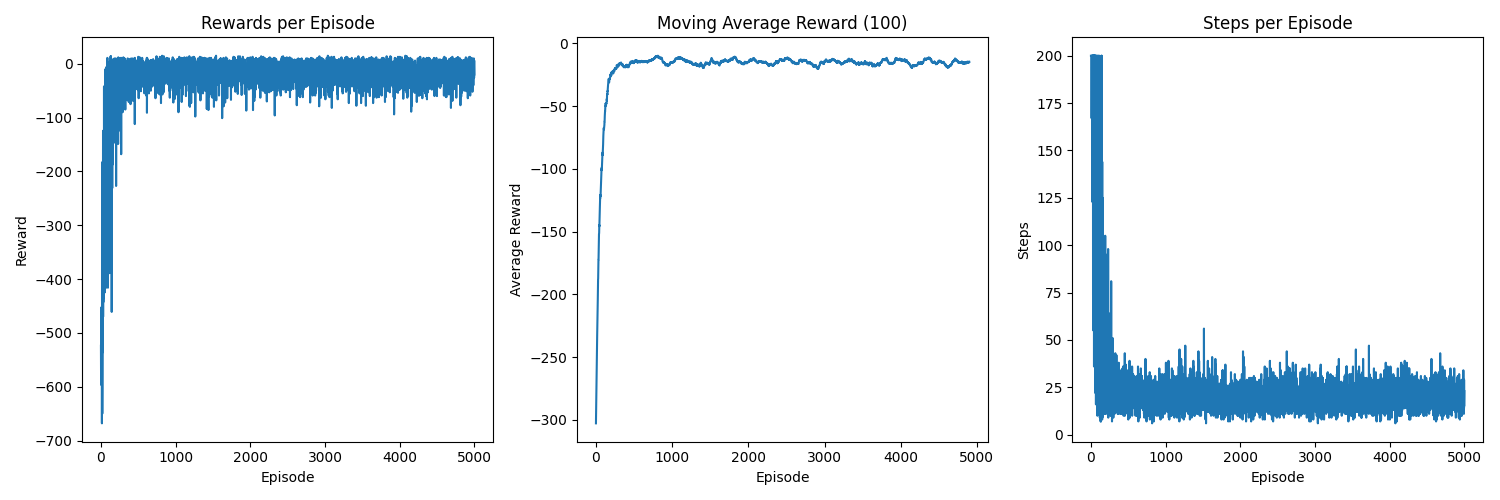
\includegraphics[width=0.7\linewidth]{images/a09g09e03d0.png}
    \caption{Taxi Q-Learning with $\alpha = 0.9$; $\gamma = 0.9$; $\epsilon = 0.3$; and no $\epsilon$-decay}
    \label{e0.3}
\end{figure}

\begin{figure}[H]
    \centering
    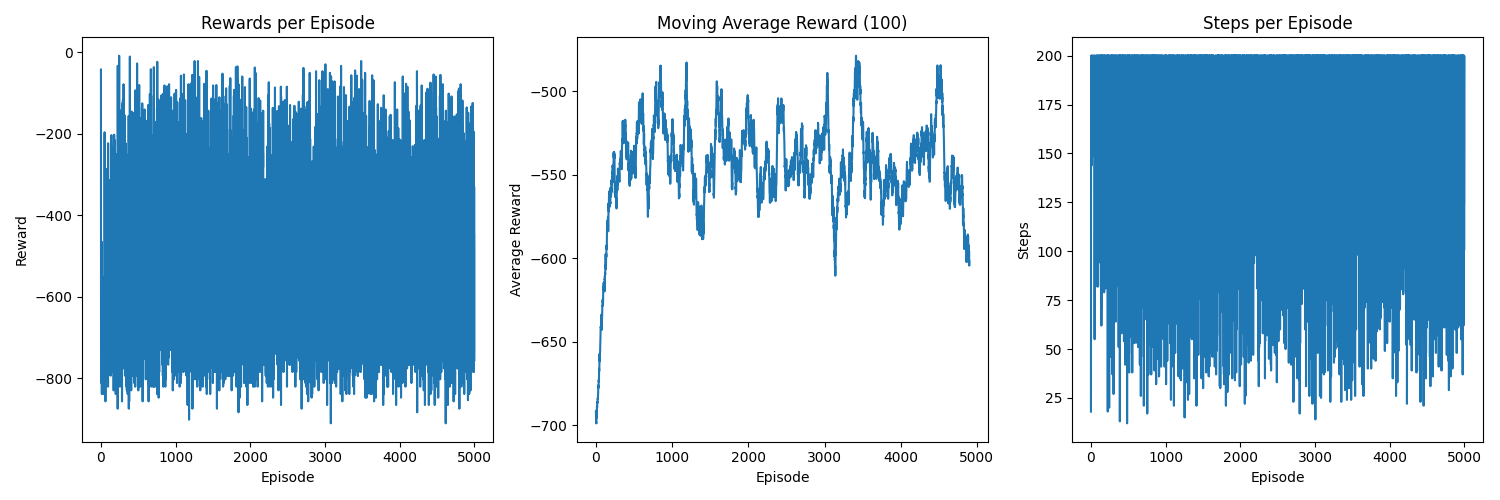
\includegraphics[width=0.7\linewidth]{images/a09g09e09d0.png}
    \caption{Taxi Q-Learning with $\alpha = 0.9$; $\gamma = 0.9$; $\epsilon = 0.9$; and no $\epsilon$-decay}
    \label{e0.9_nodecay}
\end{figure}

\begin{figure}[H]
    \centering
    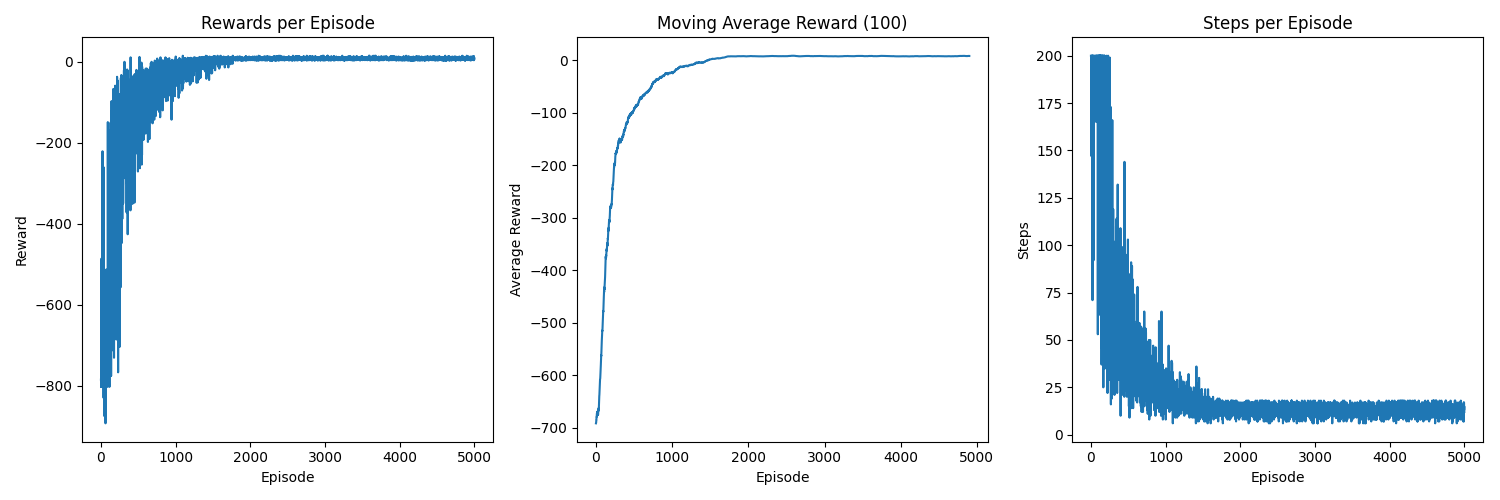
\includegraphics[width=0.7\linewidth]{images/decay-a09g09e09d0_0005.png}
    \caption{Taxi Q-Learning with $\alpha = 0.9$; $\gamma = 0.9$; $\epsilon = 0.9$; $\epsilon-decay = 0.0005$}
    \label{e0.9_decay0.0005}
\end{figure}

\begin{figure}[H]
    \centering
    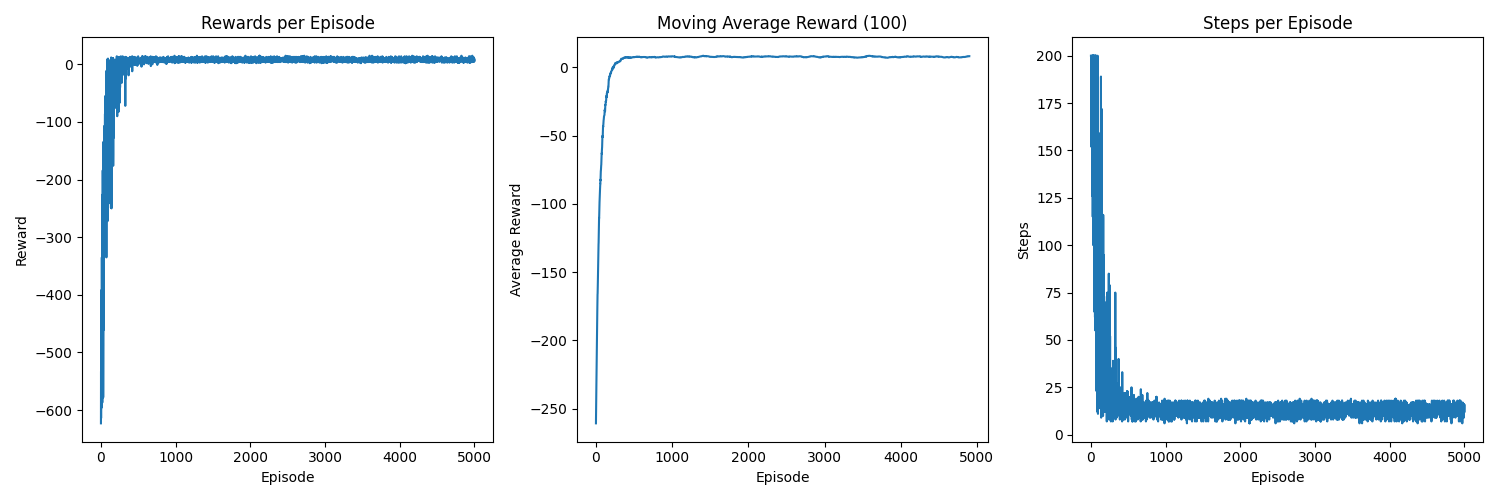
\includegraphics[width=0.7\linewidth]{images/decay-a09g09e02d0_0005.png}
    \caption{Taxi Q-Learning with $\alpha = 0.9$; $\gamma = 0.9$; $\epsilon = 0.2$; $\epsilon-decay = 0.0005$}
    \label{e0.2_decay0.0005}
\end{figure}

\begin{figure}[H]
    \centering
    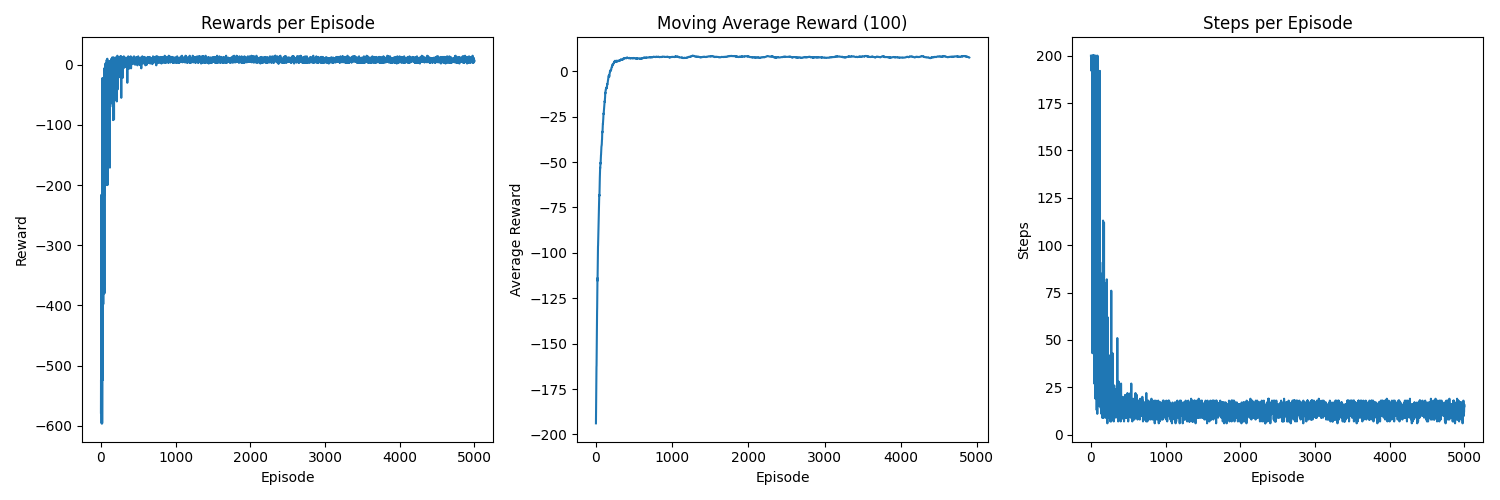
\includegraphics[width=0.7\linewidth]{images/a09g09e00d0.png}
    \caption{Taxi Q-Learning with $\alpha = 0.9$; $\gamma = 0.9$; $\epsilon = 0.0$; and no $\epsilon$-decay}
    \label{e0.0}
\end{figure}

\begin{figure}[H]
    \centering
    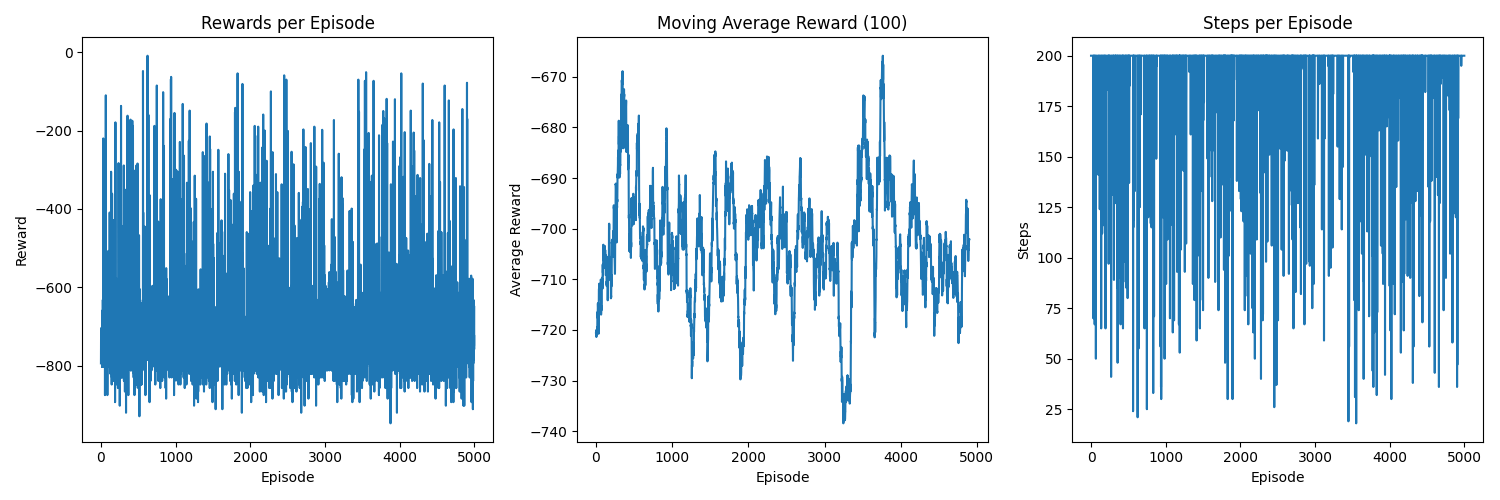
\includegraphics[width=0.7\linewidth]{images/sarsa-a09g09e09d0.png}
    \caption{Taxi SARSA with $\alpha = 0.9$; $\gamma = 0.9$; $\epsilon = 0.9$; and no $\epsilon$-decay}
    \label{sarsa}
\end{figure}

\begin{figure}[H]
    \centering
    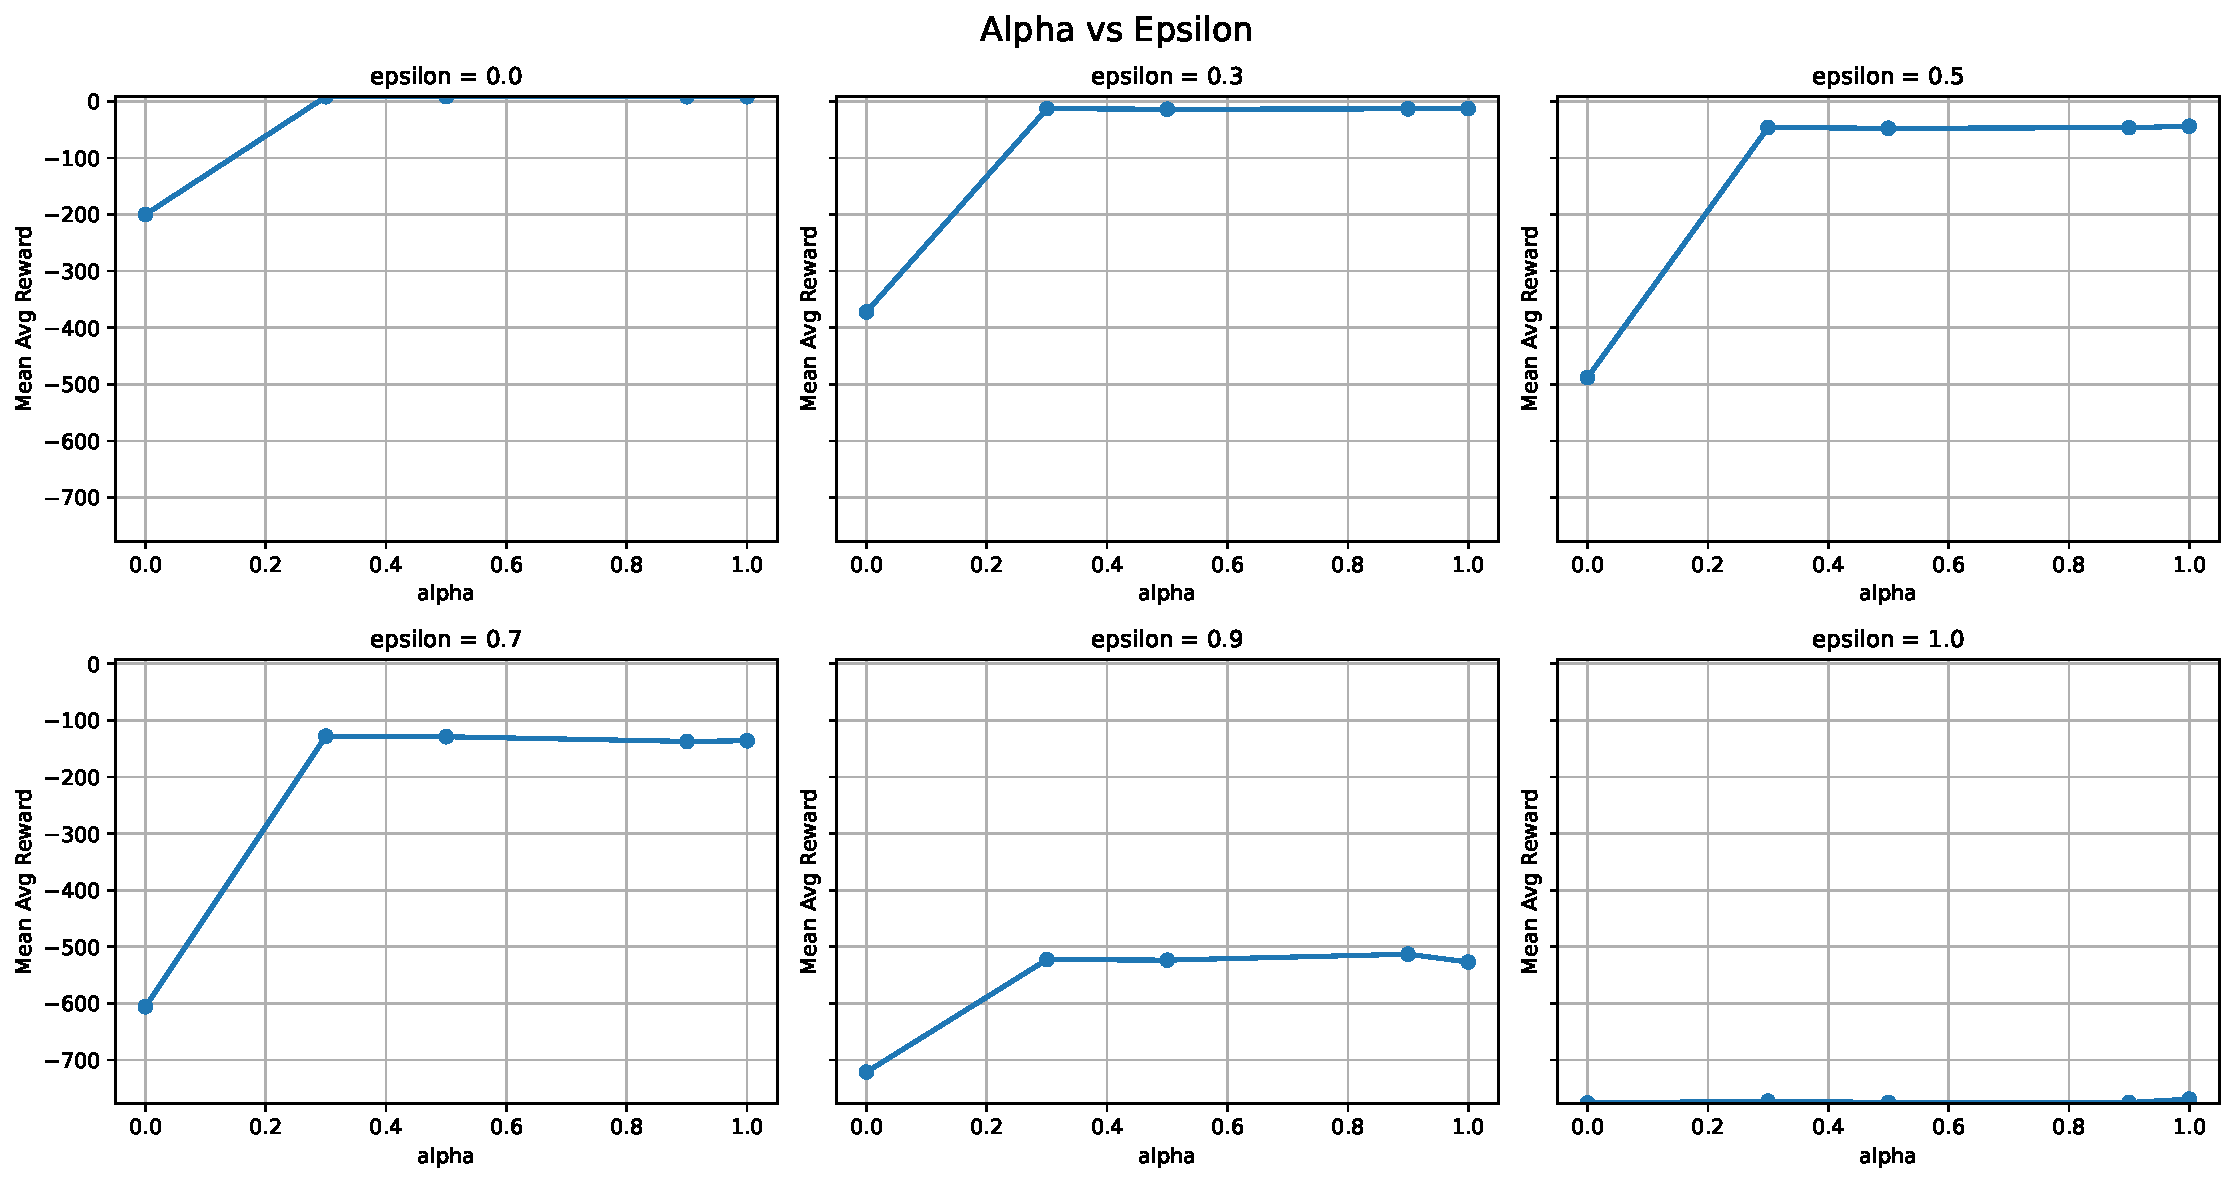
\includegraphics[width=0.8
    \linewidth]{images/alpha_vs_epsilon.pdf}
    \caption{$\alpha$ vs $\epsilon$ with fixed $\gamma = 0.9$}
    \label{alphavsepsilon}
\end{figure}

\begin{figure}[H]
    \centering
    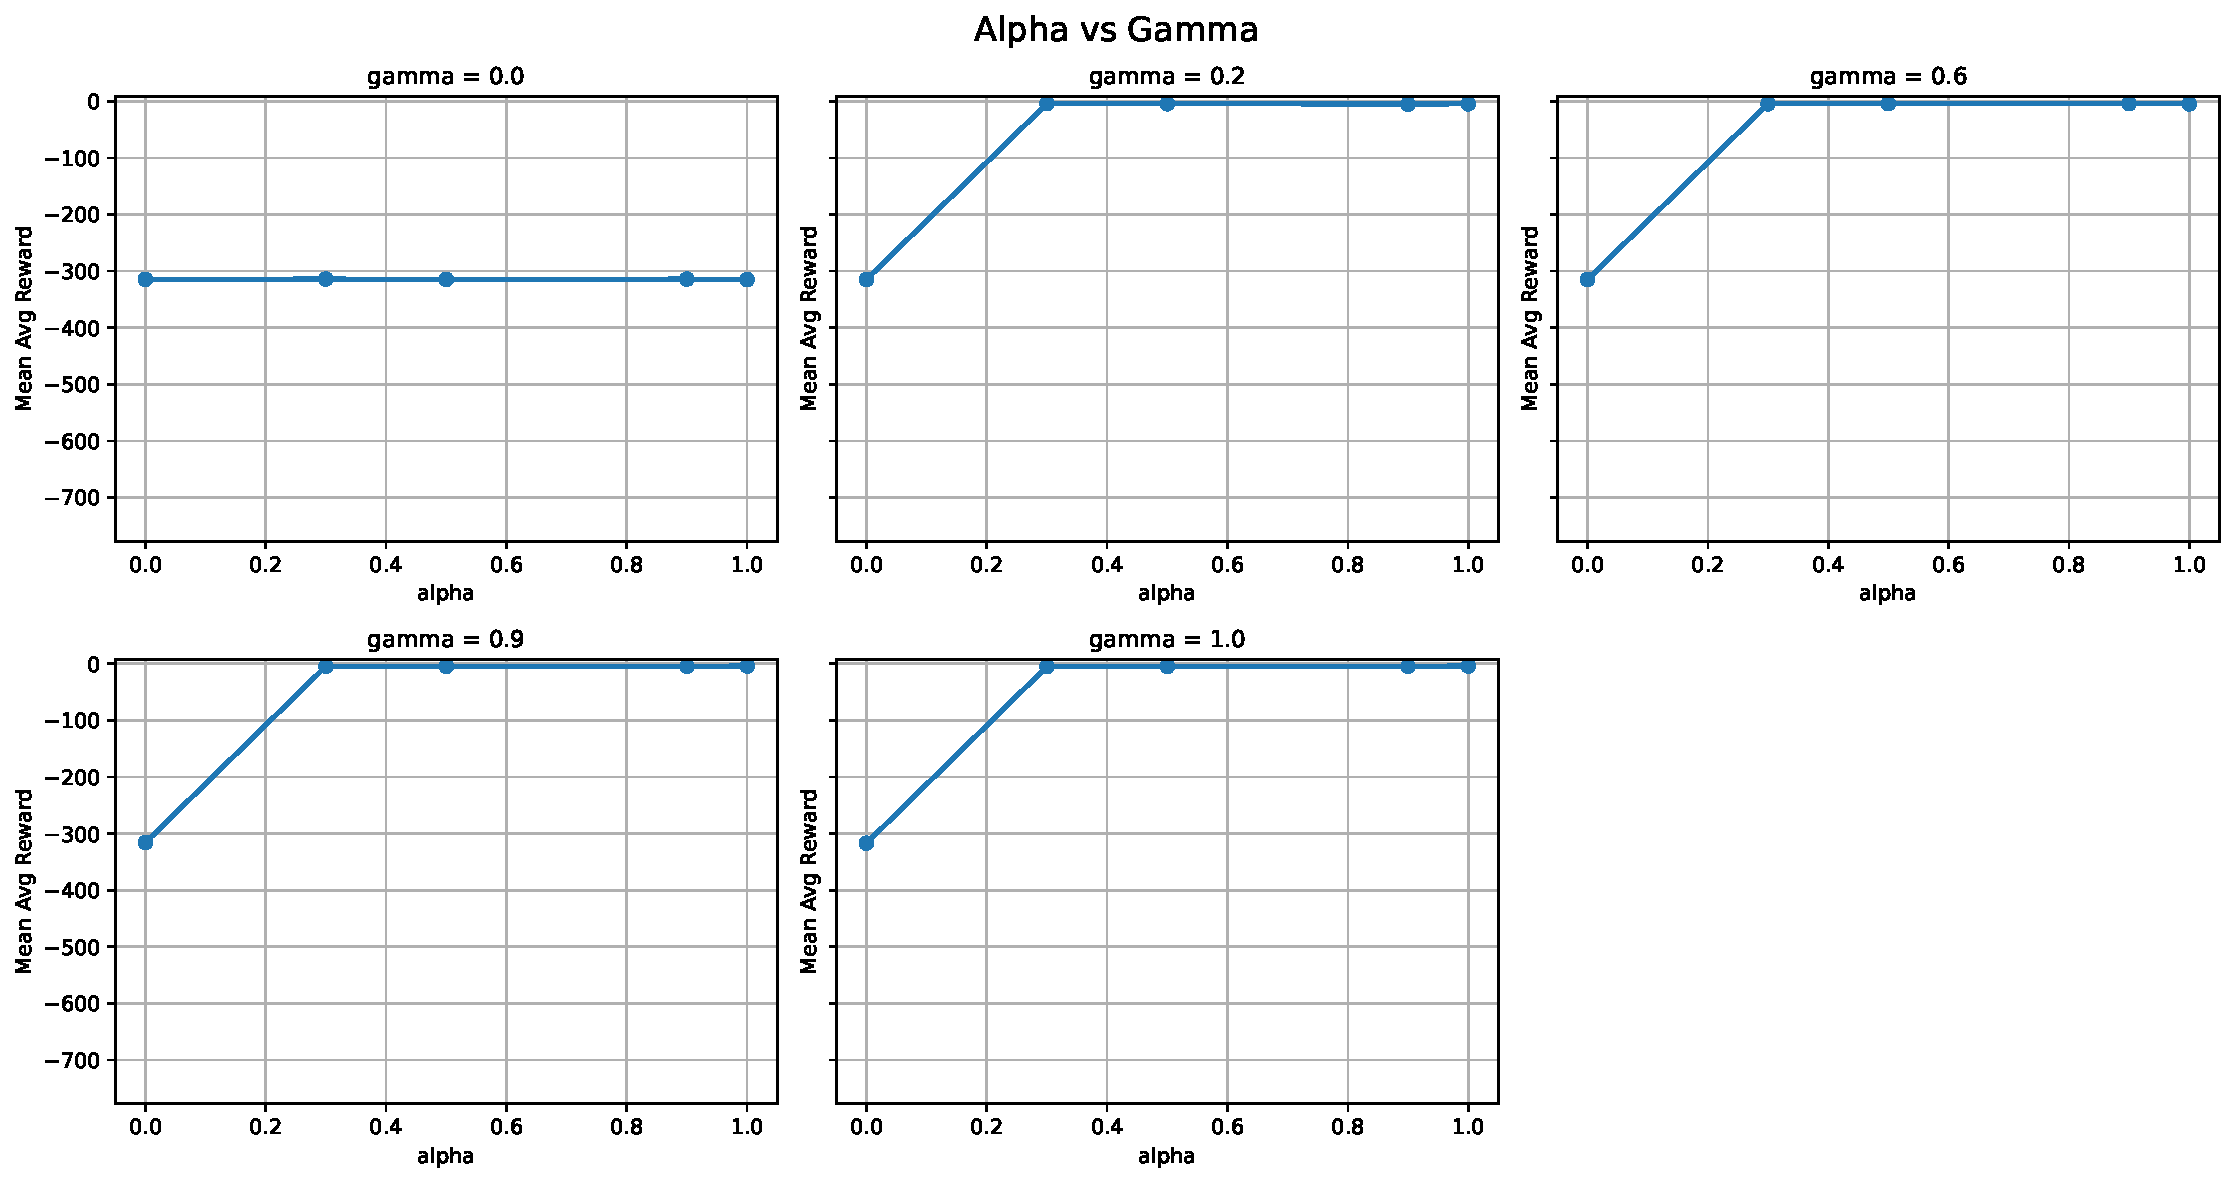
\includegraphics[width=0.8
    \linewidth]{images/alpha_vs_gamma.pdf}
    \caption{$\alpha$ vs $\epsilon$ with fixed $\epsilon = 0.2$}
    \label{alphavsgamma}
\end{figure}

\begin{figure}[H]
    \centering
    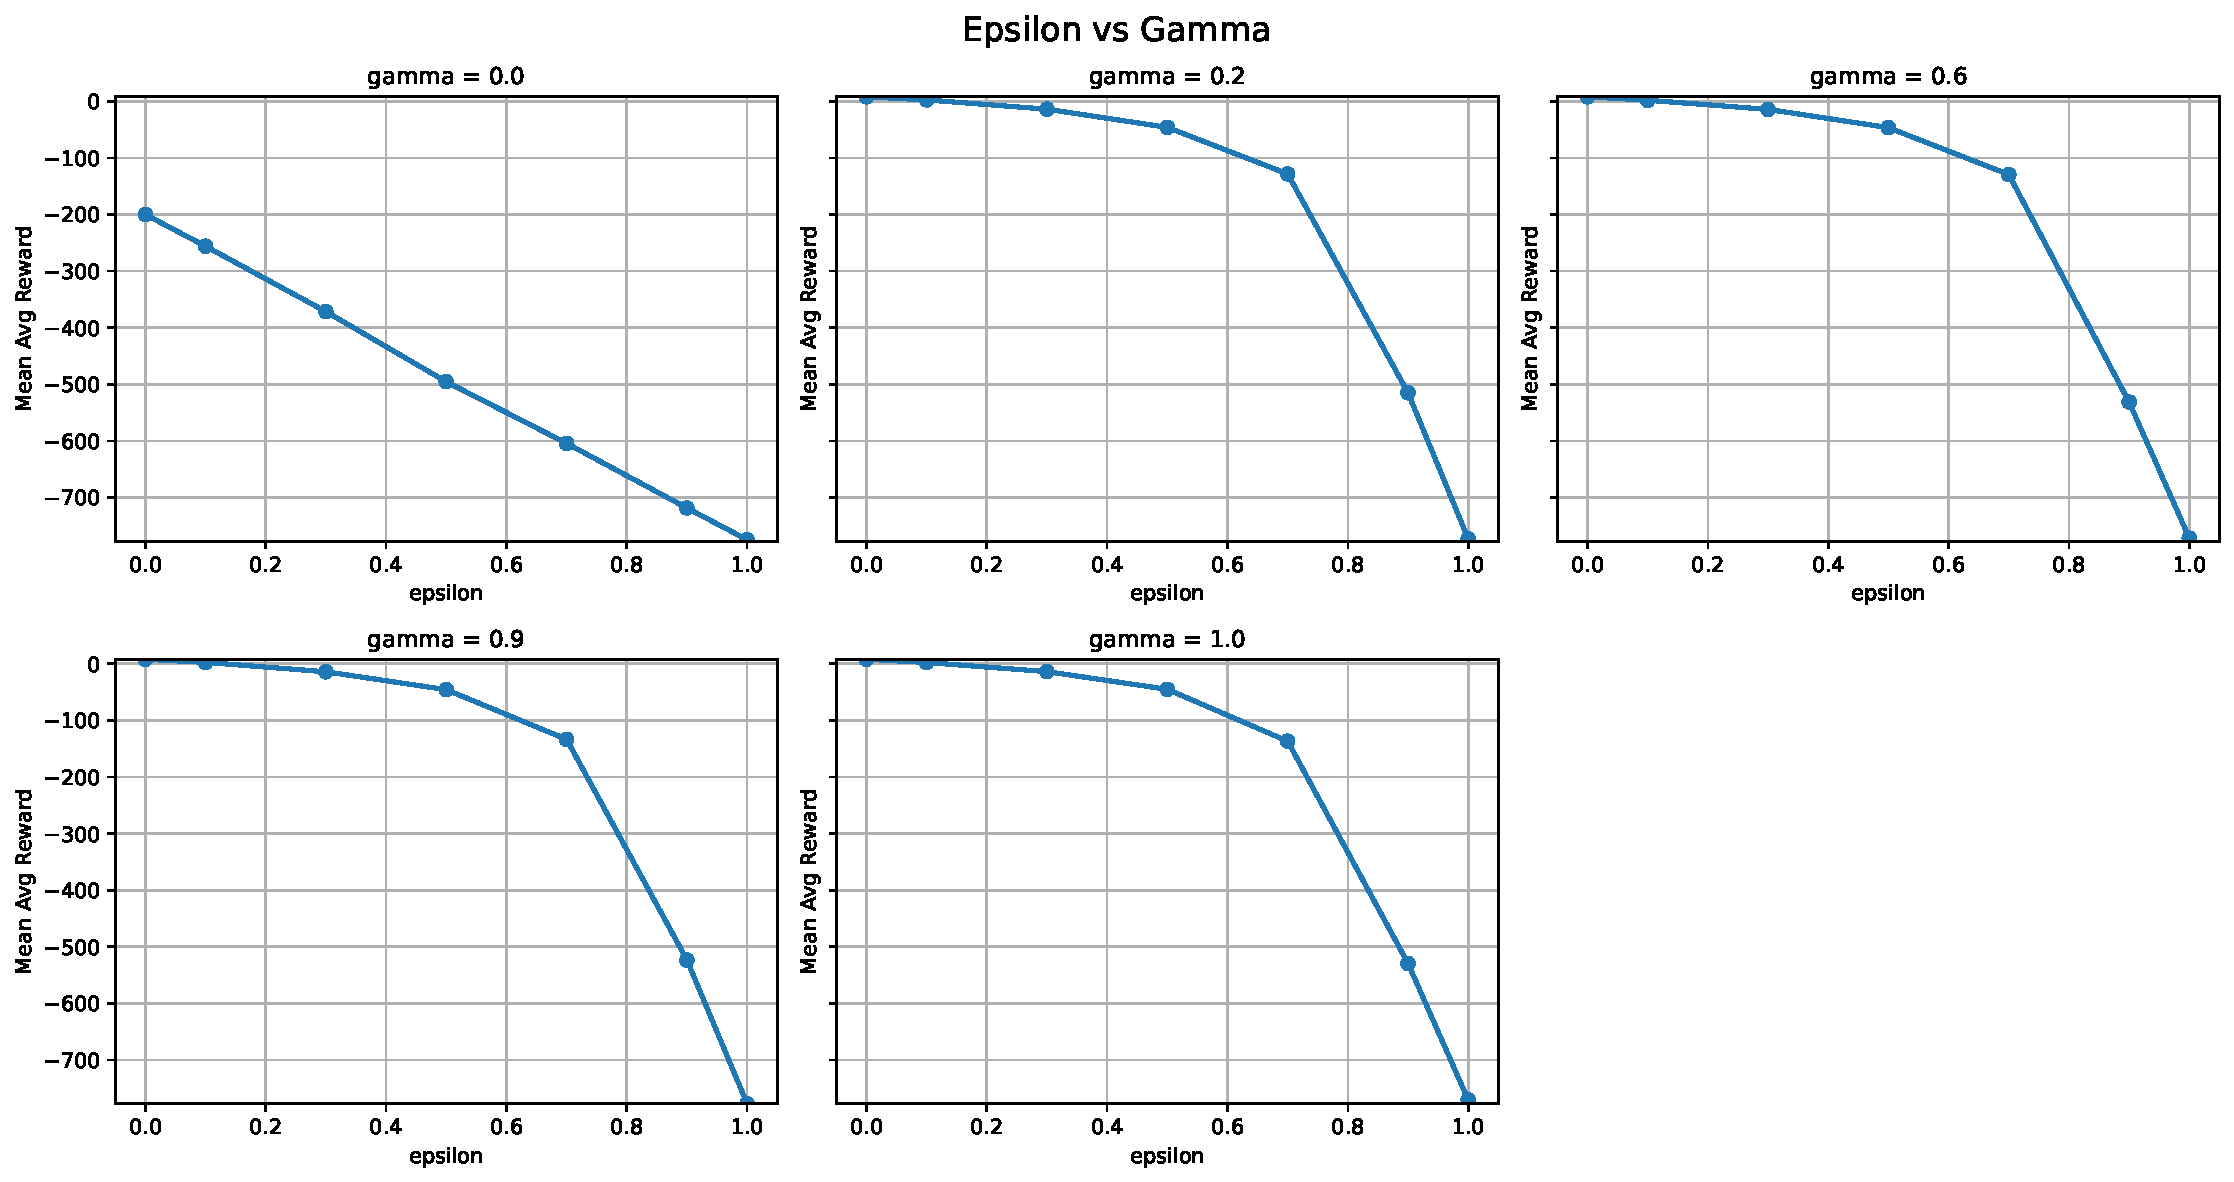
\includegraphics[width=0.8
    \linewidth]{images/epsilon_vs_gamma.pdf}
    \caption{$\alpha$ vs $\epsilon$ with fixed $\alpha = 0.3$}
    \label{epsilonvsgamma}
\end{figure}

\subsection*{Breakout DQN}

\begin{figure}[H]
    \centering
    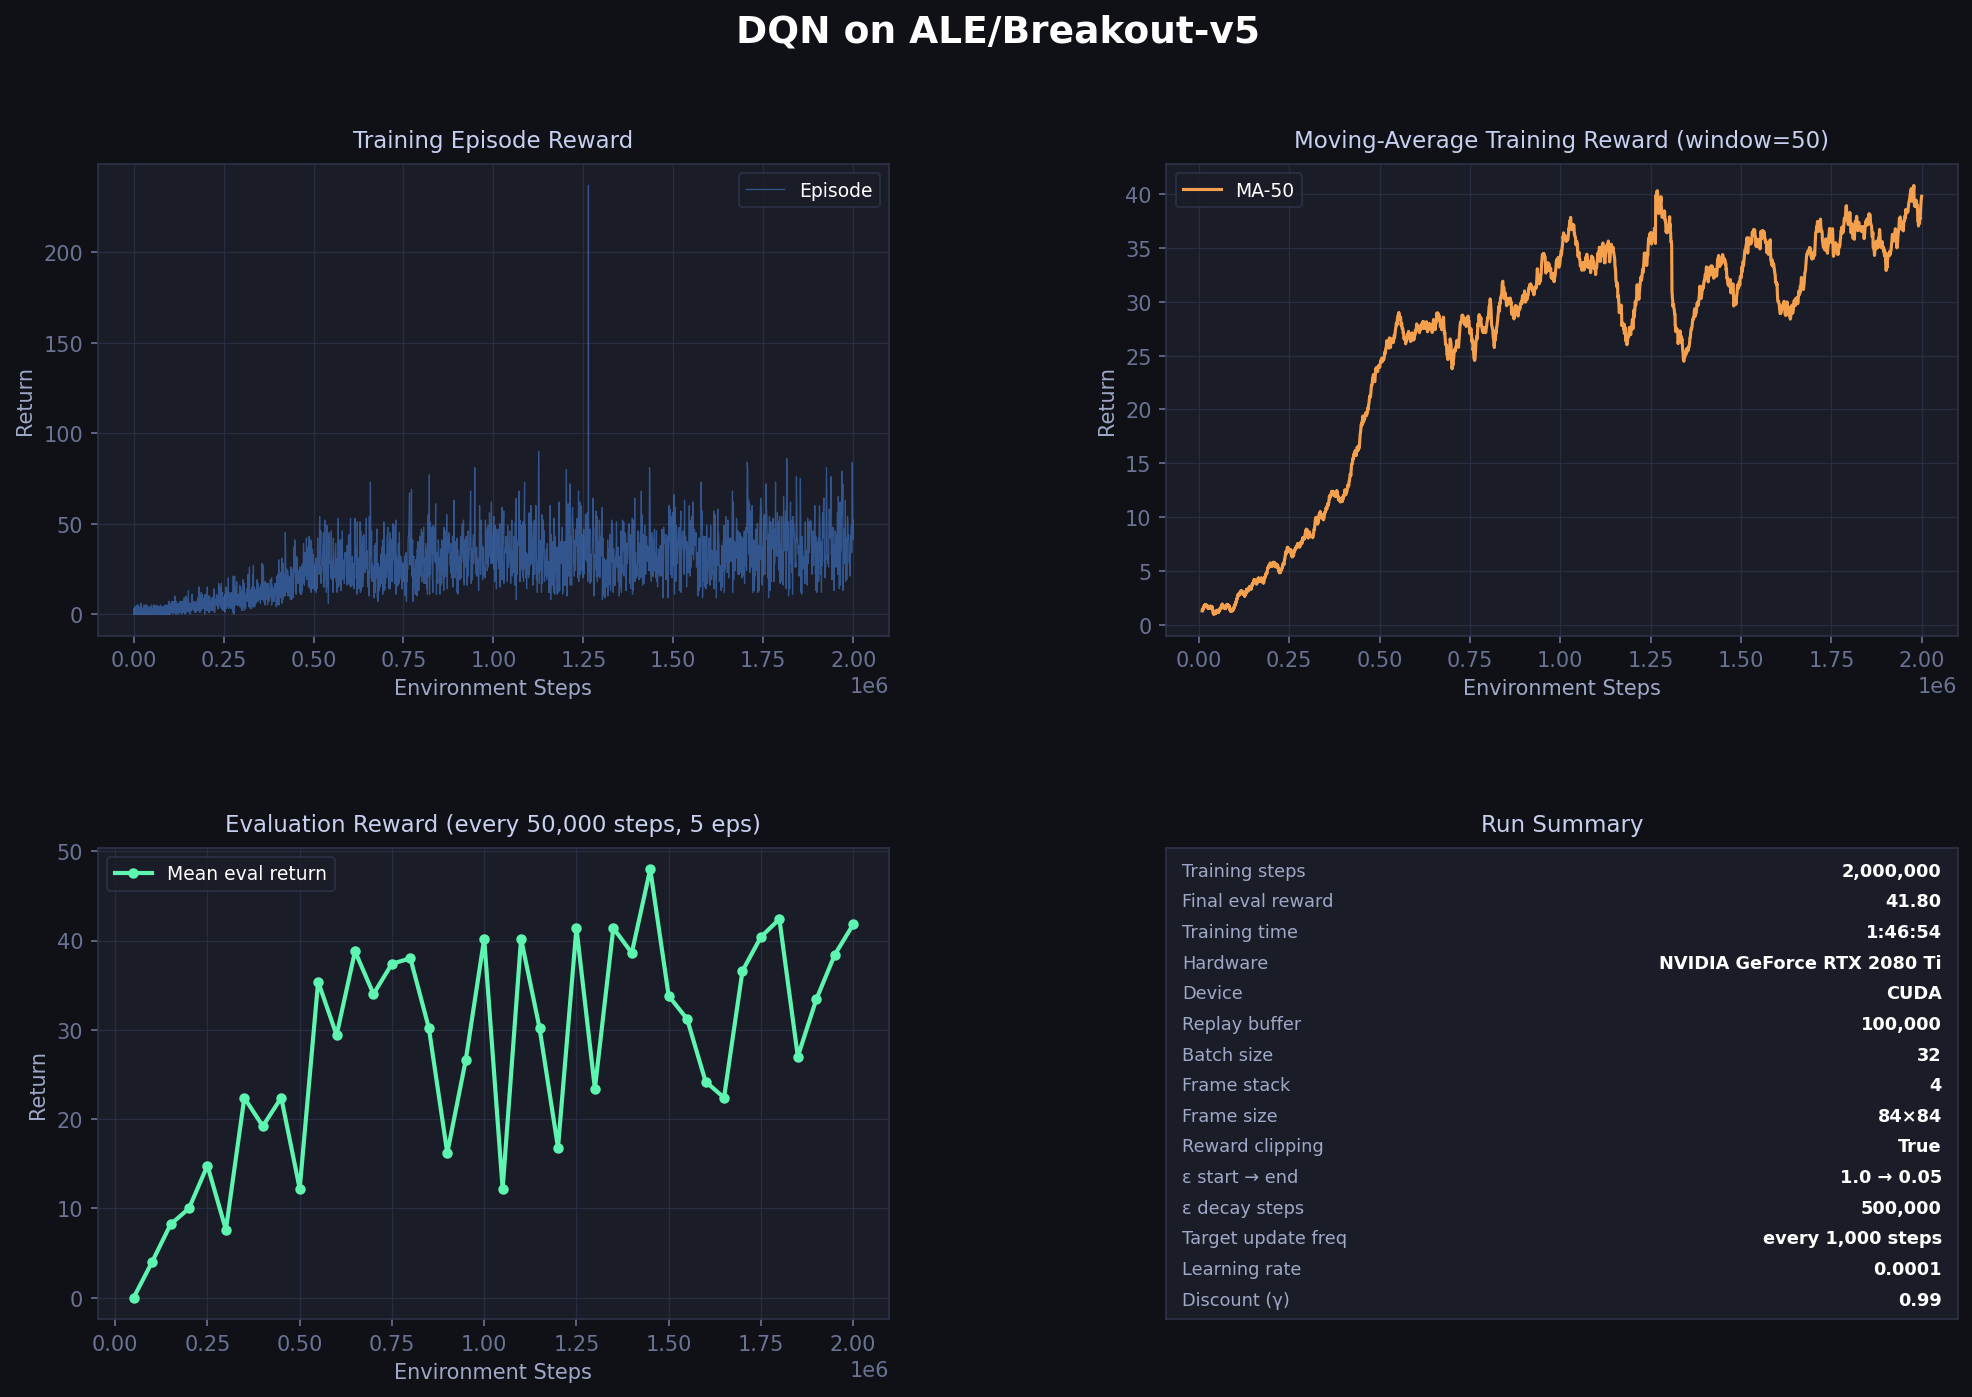
\includegraphics[width=0.7\linewidth]{images/dqn_breakout_results2m.png}
    \caption{DQN}
    \label{dqn}
\end{figure}

\section*{Comparative Analysis}

Taxi and Breakout represent fundamentally different reinforcement learning problems. Taxi is typically solved using tabular Q-learning because its state space is small, discrete, and enumerable. In contrast, Breakout requires Deep Q-Networks (DQN) since its high-dimensional image observations cannot be stored efficiently in a Q-table. Instead, DQN approximates the Q-function using a neural network.

Taxi uses structured symbolic states containing the taxi position, passenger location, and destination, allowing straightforward policy learning. Breakout instead provides raw image frames, requiring the agent to learn visual features such as ball motion, paddle position, brick locations, and collision dynamics directly from pixels, making perception and control significantly more complex.

Taxi is also far more sample efficient because its small state space allows frequent state revisitation and faster Q-value convergence. Breakout requires substantially more interactions due to its enormous state space, sparse rewards, and ineffective random exploration during early training.

From a computational perspective, Taxi is lightweight since tabular Q-learning only updates scalar Q-values. Breakout is far more computationally expensive because DQN trains deep convolutional networks alongside replay buffers and target networks, often requiring GPUs and long training times.

Learning in Taxi is generally more stable because tabular Q-learning updates exact state-action entries without function approximation. In contrast, DQN suffers from instability caused by bootstrapping, off-policy learning, and neural network approximation, known as the deadly triad. Replay buffers and target networks are therefore required to stabilize training.

Finally, Taxi policies are highly interpretable because Q-values are explicitly stored for each state-action pair. In Breakout, the policy is implicitly encoded within neural network weights, making the agent’s decision process much harder to interpret.

\begin{table}[H]
\centering
\caption{Comparison Between Taxi and Breakout}
\label{tab:taxi_breakout_comparison}

\begin{tabular}{|p{4cm}|p{4cm}|p{6.5cm}|}
\hline
\textbf{Aspect} & \centering\textbf{Taxi} & \centering\textbf{Breakout} \arraybackslash \\
\hline
Learning Method & Tabular Q-Learning & DQN \\
\hline
State & Discrete & Image-based \\
\hline
Sample Efficiency & High & Low \\
\hline
Computational Cost & Low & High \\
\hline
Stability of Learning & More stable & Less stable (deadly triad)\\
\hline
Policy Interpretability & Interpretable Q-Values & Less interpretable NN parameters \\
\hline
Main difficulty & Exploration and policy learning & Representation learning and stability \\
\hline
\end{tabular}

\end{table}

\section*{Conclusion}

The experiments executed have demonstrated how the characteristics of an environment strongly influence the choice of reinforcement learning method. In the Taxi environment, the small discrete state space, deterministic transitions, and dense rewards made tabular methods such as Q-learning and SARSA effective and computationally efficient. Experimental results showed that Q-learning achieved stable convergence and generally outperformed SARSA in this deterministic setting, while hyperparameter studies highlighted the importance of learning rate, discount factor, and exploration strategy in agent performance.

In contrast, the Breakout environment presented significantly greater challenges due to its high-dimensional image-based observations, sparse rewards, and large state space. These characteristics made tabular approaches impractical and required the use of Deep Q-Networks with function approximation. Techniques such as replay buffers, target networks, frame preprocessing, and $\epsilon$-greedy exploration were essential for stabilizing learning and enabling the agent to learn meaningful visual and control representations from raw pixels.

Overall, the comparison between Taxi and Breakout illustrates the progression from classical reinforcement learning methods to deep reinforcement learning approaches as environment complexity increases. The study highlights important trade-offs between interpretability, computational cost, sample efficiency, and learning stability, while also demonstrating how reinforcement learning combines decision-making, optimization, and representation learning to solve increasingly complex tasks.

\bibliography{references}

\end{document}